
\clearpage
\section{Extended Related Work}
\label{app:relwork}

\subsection{Detailed Comparison with the Closest Methods}
\label{app:compare}

\begin{table}[t]
\centering
\caption{\textbf{Among these methods, only \method{} repairs an external teacher without task reward and refreezes it for distillation.} RQ-free: no task-reward query for distillation supervision. The two right columns concern an external scorer, not an evolving self-teacher. $^{\dagger}$FutureBridge uses a success-selected reference pool.}
\label{tab:positioning}
\footnotesize
\setlength{\tabcolsep}{4pt}
\begin{tabular}{@{}>{\raggedright\arraybackslash}p{5.8cm}ccc@{}}
\toprule
\textbf{Method} & \textbf{RQ-free} & \shortstack{\textbf{Repairs external}\\\textbf{teacher}} & \shortstack{\textbf{Freeze, then}\\\textbf{distill}} \\
\midrule\midrule
TCOD-F2B \citep{tcod2026} & \textcolor{box_green}{\cmark} & \textcolor{gray}{\xmark} & \textcolor{gray}{\xmark} \\
Guided-OPD \citep{guidedopd2026} & \textcolor{box_green}{\cmark} & \textcolor{gray}{\xmark} & \textcolor{gray}{\xmark} \\
FutureBridge$^{\dagger}$ \citep{futurebridge2026} & \textcolor{box_green}{\cmark} & \textcolor{gray}{\xmark} & \textcolor{gray}{\xmark} \\
ReOPD \citep{reopd2026} & \textcolor{box_green}{\cmark} & \textcolor{gray}{\xmark} & \textcolor{gray}{\xmark} \\
SDFT / OPCD \citep{sdft2026,opcd2026} & \textcolor{box_green}{\cmark} & \textcolor{gray}{\xmark} & \textcolor{gray}{\xmark} \\
CANON \citep{canon2026} & \textcolor{box_green}{\cmark} & \textcolor{gray}{\xmark} & \textcolor{gray}{\xmark} \\
SDAR \citep{sdar2026} & \textcolor{gray}{\xmark} & \textcolor{gray}{\xmark} & \textcolor{gray}{\xmark} \\
Distillation Traps and Guards \citep{trapsguards2026} & \textcolor{gray}{\xmark} & \textcolor{box_green}{\cmark} & \textcolor{box_green}{\cmark} \\
\midrule
\textbf{\method{} (ours)} & \textcolor{box_green}{\cmark} & \textcolor{box_green}{\cmark} & \textcolor{box_green}{\cmark} \\
\bottomrule
\end{tabular}
\end{table}


\Cref{tab:positioning} places the compared methods by the three properties in its columns; updating an EMA self-teacher during actor training is different from this separate scorer-repair stage.

\textbf{Student-side curricula.} TCOD-F2B~\citep{tcod2026} gradually lengthens the student's training episodes. Guided-OPD~\citep{guidedopd2026} assigns a decreasing share of turns to the teacher, combining cross-entropy on teacher tokens with distillation on student tokens. ReOPD~\citep{reopd2026} replays pre-collected teacher prefixes. All three leave the external scorer unchanged; a repaired teacher can supply scores under such curricula as well as under ordinary OPD.

\textbf{FutureBridge and teacher continuations.} FutureBridge~\citep{futurebridge2026} is our closest experimental comparator. It continues from high-disagreement student states and validates a bridge with short student rollouts; accepted teacher text enters the student's training buffer, alongside a curriculum over success-selected reference prefixes. Its online acceptance rule reads no task reward, although the reference pool uses success selection. \method{} instead uses a selected takeover as privileged context for teacher repair: the teacher learns to reproduce its informed scores without that context and is then frozen, and the student retains ordinary OPD.

\textbf{Privileged context and consensus.} SDFT~\citep{sdft2026} and Self-Distilled Reasoner~\citep{opsd2026} train an acting model from a demonstration-conditioned self-teacher. OPCD~\citep{opcd2026} also supports an external context-conditioned teacher, but transfers the context into the student directly. CANON~\citep{canon2026} supplies a label-free reference by selecting the solution with the majority answer. Our consensus selection follows this principle, applied to an external teacher's continuations from student states; the model being fitted becomes the scorer of a subsequent distillation stage.

\textbf{Feedback and reward-based learning.} SDPO~\citep{sdpo2026} turns rich environment feedback into self-distillation targets, and in scalar-feedback settings uses successful attempts as feedback. SDAR~\citep{sdar2026} is a multi-turn hybrid that keeps reward-based RL as its primary objective and adds gated self-distillation. We exclude this additional student reward signal from the experimental comparison; \method{} could supply the distillation scorer of such a hybrid.

\textbf{External teacher calibration.} Distillation Traps and Guards~\citep{trapsguards2026} also changes the teacher before distillation, by reinforcement fine-tuning with utility and calibration rewards and a KL anchor; \method{} instead fits takeover-informed soft targets on student histories through the cross-entropy of \Cref{eq:r2s}, without task reward.

\subsection{Further Related Work}
\label{app:related}

\textbf{OPD at scale.} MiMo-V2-Flash integrates domain-specialized teachers with dense token-level supervision~\citep{mimo2026}, and Nemotron-Cascade 2 uses multi-domain OPD between Cascade RL stages to recover capabilities from the strongest intermediate domain checkpoints~\citep{nemotroncascade22026}. Our question concerns the quality of the next-token supervision a given teacher supplies on multi-turn student histories.

\textbf{Other ways to adapt a model.} OPD is one of several routes from a pretrained model to a task. Fine-tuning adapts the weights on fixed data, through low-rank adapters, knowledge-anchored low-resource adaptation or prompt-based continual learning~\citep{zhao2026mora,zhao2025kalahash,zhao2024reconstruct,zou2025learning}; RL adapts them on task reward, as in ParallelSearch for search agents~\citep{zhao2025parallelsearch}; in-context learning leaves the weights fixed and adapts through examples, including self-mined errors~\citep{zhao2026value}; and task-specific models are built for one domain~\citep{hao2025safemap}. Agentic OPD differs from all four in its signal: a teacher's next-token distribution on the student's own trajectories, scored while the student acts.

\textbf{Local supervision and privileged information.} Beyond the compatibility and privileged-context findings of \citet{li2026bestval} and \citet{rethinkingopsd2026} discussed in \Cref{sec:related}, Multi-Rollout OPD~\citep{mropd2026} enriches the teacher's context with peer attempts labelled by success or failure. Our references are teacher takeovers from the student's own state, selected without task reward and internalized into an external scorer, which we assess through target fidelity and the completion behavior of its distilled students.


\section{Analysis Details}
\label{app:analysis}
\label{app:delay}

\begin{table}[t]
\centering
\caption{\textbf{The states and scores behind \Cref{tab:drift}.} \emph{All}: the untrained student's highest-disagreement states with a replayable takeover; \emph{Turn $\geq 5$}: those from turn five on, which \Cref{tab:drift} uses; \emph{Lost}: of these, the states the student went on to lose. \emph{Scored}: states where at least one takeover finishes, and the student's turns through the mined one, which the drop columns read. \emph{Against other}: a class's mean change in log-probability over that of the rest of the thinking, with a 95\% interval over states; \emph{Drop}: as in \Cref{tab:drift}, for the student's committing words and its action tokens.}
\label{tab:drift-detail}
\footnotesize
\setlength{\tabcolsep}{3.5pt}
\begin{tabular}{@{}lccccccccc@{}}
\toprule
& \multicolumn{3}{c}{States} & \multicolumn{2}{c}{Scored} & \multicolumn{2}{c}{Against other} & \multicolumn{2}{c}{Drop (\%)} \\
\cmidrule(lr){2-4}\cmidrule(lr){5-6}\cmidrule(lr){7-8}\cmidrule(l){9-10}
Environment & All & Turn $\geq 5$ & Lost & States & Turns & Hedging & Searching & Committing & Action \\
\midrule\midrule
ALFWorld & 2,399 & 814 & 489 & 458 & 4,957 & $2.4$ $[2.1, 2.8]$ & $1.8$ $[1.4, 2.2]$ & $6.1$ & $0.1$ \\
WebShop & 2,398 & 689 & 647 & 107 & 906 & $2.0$ $[1.3, 2.9]$ & $1.9$ $[0.9, 3.0]$ & $6.8$ & $0.5$ \\
ScienceWorld & 2,205 & 682 & 555 & 403 & 4,085 & $2.7$ $[2.4, 3.1]$ & $3.5$ $[3.0, 4.1]$ & $11.3$ & $0.3$ \\
\bottomrule
\end{tabular}
\end{table}


\textbf{The table of \Cref{sec:takeover}.} \Cref{tab:drift} uses the untrained student's highest-disagreement states from turn five on, where a takeover is no longer close to the teacher acting alone from the start; \Cref{tab:drift-detail} counts them. Success is the environment's own outcome. The drop columns keep the states where at least one takeover finishes and read the student's turns up to and including the mined one. The teacher scores the student's own tokens twice, plain and with that takeover in context, as described in \Cref{app:r2s}; a drop entry is $100\,(1-e^{\bar d})$, where $\bar d$ is the mean change in log-probability over the student's tokens of that kind. Hedging words are the thinking tokens \emph{maybe, might, likely, probably, perhaps, could, possibly, seem(s), guess, assume, unsure, potentially, whether, if, unless, unclear, unknown, hopefully, presumably}; searching words are \emph{look, search, check, examine, explore, find, locate, scan, browse} with their inflections, and \emph{inventory}; \emph{other} is the rest of the thinking. \Cref{tab:drift-detail} also gives, with 95\% intervals over states, how much more each class falls than the rest of the thinking, and the drop on the student's words of committing (\emph{take, put, use, buy, now, done}, \ldots), which fall less than its hedging words and more than the rest, and on its action tokens, which barely move.

\begin{table}[t]
\centering
\caption{\textbf{The teacher's takeovers finish from the student's states in every cell.} Success (\%) of the untrained student and of the teacher's $K{=}8$ takeovers over all mined states, for every pair of \Cref{tab:main}.}
\label{tab:takeover-all}
\small
\setlength{\tabcolsep}{4.5pt}
\begin{tabular}{@{}lcccccc@{}}
\toprule
\multirow{2}{*}{Teacher $\to$ student} & \multicolumn{2}{c}{ALFWorld} & \multicolumn{2}{c}{WebShop} & \multicolumn{2}{c}{ScienceWorld} \\
\cmidrule(lr){2-3}\cmidrule(lr){4-5}\cmidrule(l){6-7}
 & Student & Takeover & Student & Takeover & Student & Takeover \\
\midrule\midrule
Qwen3.5-9B$\to$2B & $11.9$ & $54.6$ & $5.0$ & $21.8$ & $1.2$ & $31.2$ \\
Qwen3.5-9B$\to$4B & $51.8$ & $56.7$ & $19.6$ & $22.0$ & $22.4$ & $35.6$ \\
Qwen3-30B-A3B$\to$4B & $33.3$ & $41.8$ & $10.4$ & $14.0$ & $10.2$ & $36.6$ \\
Qwen3-30B-A3B$\to$8B & $45.5$ & $42.2$ & $20.1$ & $31.7$ & $21.6$ & $38.8$ \\
\bottomrule
\end{tabular}
\end{table}


\textbf{The takeovers of every pair.} \Cref{tab:takeover-all} repeats the student-versus-takeover comparison of \Cref{tab:drift} for every cell of \Cref{tab:main}, over all mined states rather than those from turn five on; both entries of its Qwen3.5-9B$\to$4B row are therefore above the matching entries of \Cref{tab:drift}, since the earlier states are easier for the student and for the teacher alike. The $K{=}8$ takeovers beat the student's own outcome in eleven of twelve cells; the exception is the Qwen3-8B student on ALFWorld, which already beats its teacher acting alone and which \method{} still lifts ten points above vanilla OPD. On WebShop the 30B-A3B teacher, which seldom finishes from the first turn, finishes $14\%$ and $32\%$ of its takeovers from the students' states.

\textbf{How the episodes end.} The out-of-turn shares that \Cref{sec:takeover} cites are those of \Cref{fig:scorer-effect} and \Cref{tab:timeouts}: held-out evaluation episodes that reach the turn budget unfinished, for the 9B-taught 4B students of \Cref{tab:main} at their final checkpoint, in the three decodes behind their success there; \Cref{fig:scorer-effect} averages the seen and unseen splits, \Cref{tab:timeouts} reports the seen split.

\textbf{The \method{} student spends fewer turns searching.} \Cref{tab:search-turns} reads the students' own training rollouts in the last ten updates of each run. \emph{Searching} counts the turns spent moving, opening and looking (ALFWorld: go to, open, close, look, examine, inventory; ScienceWorld: teleport, look, read, wait, open, close; WebShop: search, next or previous page, back to search); \emph{task} counts the turns spent acting on the goal (ALFWorld: take, move, put, clean, heat, cool, use; ScienceWorld: focus, pick up, move, pour, use, activate, connect and the like; WebShop: opening an item, choosing an option, reading its description, buying). The win-only counts of \Cref{sec:exp-longhorizon} are averaged over the three runs in the same way.

\section{\method{} Implementation Details}
\label{app:r2s}

\textbf{Untrained-student episodes.} Before training, the untrained student plays the training-split tasks under the training prompt at $T{=}1.0$, for the episode budget of a training run (150 steps); evaluation tasks are discarded before scoring.

\textbf{Mining score.} In $\Delta_t$ of \Cref{eq:divscore}, $\student$ is the untrained student, and each term is the sampled per-token estimate of the reverse KL of \Cref{eq:opd}, so a single token's term can take either sign. Action tokens stay out of $\Delta_t$ because the thinking before them decides the action; with a finishing takeover in context, the teacher's scores of the student's action tokens barely move, as \Cref{tab:drift-detail} shows.

\textbf{Filters and mining.} A turn is eligible when its thinking span has at least three tokens and when it ends in a tool call. Within each episode we keep the eligible turn with the largest $\Delta_t$ (one state per episode), cap three states per goal, and keep the top $N{=}2{,}400$ states by $\Delta_t$. A state is dropped when its prompt cannot be re-tokenized identically, when its privileged stream exceeds $32{,}768$ tokens, or when it has no privileged position.

\textbf{Takeovers.} From each restored state the teacher attempts the episode $K{=}8$ times independently, sampled at $T{=}1.0$ with reasoning mode off, up to the environment's turn budget. \Cref{tab:takeover-all} gives the takeover success of every cell of \Cref{tab:main}; between $2{,}159$ and $2{,}400$ of a cell's mined states have at least one replayable takeover, and at least one of the eight takeovers finishes in $28$--$83\%$ of them, depending on the cell.

\textbf{Selection.} We use two reward-free checks. The consensus vote groups a state's takeovers by how they end and keeps the state when the largest group holds at least $m$ of them; the LLM judge, Qwen3.5-9B with reasoning mode on, reads each takeover and keeps the state when it approves at least $m{=}1$. For \Cref{tab:main}, the vote uses $m{=}2$ on ALFWorld, over the takeovers that end within the turn budget, and $m{=}1$ on ScienceWorld, over those that end with the environment's completion message; on WebShop the judge checks each purchase against the instruction, for both teachers, and the approved takeovers are grouped by the item bought. The shortest takeover of the largest group is selected. In \Cref{tab:selection}, the consensus row votes with $m{=}2$ everywhere, and on ALFWorld and ScienceWorld the judge row reads the whole episode but never the reward or the completion message, and takes the shortest approved takeover. Only the ground-truth row of \Cref{tab:selection} reads the task reward.

\textbf{Privileged targets and plain scores.} The frozen teacher $T_0$ scores the student's unmodified token stream through the end of the episode. In the privileged pass the selected takeover is inserted as one extra user message immediately before the student's first turn. The message is headed ``Reference walkthrough'' and lists the teacher's thinking and action for each takeover step, without the replayed prefix and without environment observations; the header presents it as a successful expert completion of the same task. Every position of the student stream shifts by one constant offset, so the two passes align position by position. The plain pass scores the same stream without the message. Both passes cache per-position top-16 (token, log-probability) lists. Every assistant position from the mined turn, inclusive, to the student's final assistant turn receives $q^+$, including assistant turns without a tool call; earlier history remains causal context, and prompts and environment observations are not targets. \method{} trains only on the privileged targets; the plain pass is the reference of the drop columns of \Cref{tab:drift}.

\textbf{Loss and fine-tuning.} The loss at each labeled position is the cross-entropy between the target $q^+$, kept on its top-16 tokens and renormalized, and the model's full-vocabulary log-softmax. The targets are computed once from the frozen $T_0$ and are not recomputed as $T_\phi$ trains. As in \Cref{eq:r2s}, we average all selected assistant positions within each state, then average states. The teacher is initialized from $T_0$ and fine-tuned full-parameter for one epoch at learning rate $2\times10^{-6}$, with AdamW (betas $0.9/0.95$, no weight decay), 10 warmup steps followed by cosine decay to $0.1\times$, gradient clip 1.0, batches of 8 labeled states and bf16; 10\% of goals form a goal-disjoint held-out split. For Qwen3.5-9B the vision tower stays frozen, so full-parameter means the text decoder. The label-SFT control of \Cref{tab:abl-components} uses the same recipe. The repaired teacher is then refrozen and scores otherwise ordinary OPD in place of $T_0$, with the sampled estimator of \Cref{eq:opd-sampled}; the original teacher takes no part in the student's training.

\textbf{Self-distillation.} In \Cref{tab:self,tab:self-full}, teacher and untrained student are the same Qwen3.5-4B checkpoint, so $\Delta_t$ of \Cref{eq:divscore} is zero up to numerical noise and cannot rank states. The self pipeline instead draws one eligible turn per episode of the untrained student at random, under the same goal cap and budget, and the 4B itself runs the takeovers and the selection, so no larger model enters the pipeline. Repair and distillation follow the settings above. The vanilla control, TCOD-F2B, Guided-OPD and FutureBridge learn from the unrepaired 4B teacher; the Student alone column is the untrained 4B of \Cref{tab:main,tab:main-full}.

\section{Experimental Protocol}
\label{app:protocol}

\textbf{Environments.} WebShop~\citep{webshop2022} reports success on the 500 canonical evaluation goals and on a disjoint 256-goal pool. ALFWorld~\citep{alfworld2021} reports seen and unseen success on its held-out games under a TCOD-aligned full-history protocol; our wrapper ends an episode only on success. ScienceWorld~\citep{scienceworld2022} follows the TCOD splits: the first half of each of the 17 training task types' variations trains, 140 variations sampled from the second half form the seen evaluation, and the first 134 rows of the frozen 1{,}308-task test set of unseen types form the unseen evaluation; the metric is the simulator's completion flag, and the simulator and the action and object lists shown to the agent are TCOD's.

\textbf{Models.} The models are those of \Cref{sec:exp-setup}. Model and tokenizer revisions, prompts, environment wrappers and checkpoint provenance are in the code release, tag \texttt{r2s} of \href{https://github.com/Tree-Shu-Zhao/miles-agent}{\nolinkurl{github.com/Tree-Shu-Zhao/miles-agent}}; its 24 checkpoints are on the Hugging Face Hub.

\textbf{Prompt protocol.} Every arm and anchor of \Cref{tab:main} uses one prompt per environment, rendered in each model's native tool-call template; the prompt asks for one to three sentences of plain-text deliberation before exactly one tool call per turn, and that deliberation stays part of the generated response.

\textbf{Objective.} The vanilla OPD, \method{} and TCOD-F2B rows of \Cref{tab:main} minimize the reverse KL of \Cref{eq:opd} with its sampled estimator, which gives each student token the advantage~\citep{mimo2026,li2026bestval}
\begin{equation}
\label{eq:opd-sampled}
A_{t,i}=-\beta\!\left[\log \student(y_{t,i}\mid h_{t,i})-\log \teacher(y_{t,i}\mid h_{t,i})\right],
\qquad \tau\sim\student,
\end{equation}
with coefficient $\beta{=}1$, observations loss-masked and updates restricted to student tokens. Guided-OPD selects the teacher or the student to act at each turn and trains the student with cross-entropy on teacher-generated tokens and the same sampled reverse KL on student-generated tokens; FutureBridge applies the same sampled reverse KL to episodes that carry an accepted teacher bridge. Task reward is logged and zeroed for every distillation arm.

\textbf{Training.} Every distillation run takes 150 optimization steps and evaluates every 25 steps; the 128 WebShop episodes per step are $16$ goals $\times$ $8$ samples. Adam uses betas $(0.9, 0.98)$, weight decay 0.1 and gradient clip 1.0, and the PPO ratio clip is 0.2. TCOD-F2B, Guided-OPD and FutureBridge share this protocol and keep their own method settings.

\textbf{Evaluation.} Student-alone anchors are three decodes of the untrained student under the same prompt. An evaluation in which an episode returned no outcome after an infrastructure failure is repeated at unchanged weights and decoding seed.

\textbf{Teacher acting alone.} The teacher itself is evaluated as the acting policy at $T{=}0.4$; its split means are the teacher-alone anchors of \Cref{tab:main}, and \Cref{tab:main-full} gives them per split.

\section{Every Split of the Main Results}
\label{app:results}
\label{app:splits}

\textbf{The main text averages the splits.} Each cell of \Cref{tab:main} and \Cref{tab:self} is, per decoding seed, the mean of the seen and unseen values of the same evaluation (ALFWorld, ScienceWorld) or the success rate on the 500 canonical WebShop goals; the mean and std are then taken over the three decoding seeds. \Cref{tab:main-full} and \Cref{tab:self-full} give every split, and for WebShop also the disjoint 256-goal pool. \method{} exceeds every baseline in mean on all $24$ splits.

\begin{table}[t]
\centering
\caption{\textbf{Main results by split.} The cells of \Cref{tab:main} before averaging: ALFWorld and ScienceWorld seen\,/\,unseen, WebShop the 500 canonical goals\,/\,the disjoint 256-goal pool; protocol as in \Cref{tab:main}. Bold: the best of the five trained arms where its gap to the runner-up exceeds the larger decode std; ties are unmarked.}
\label{tab:main-full}
\scriptsize
\setlength{\tabcolsep}{3.5pt}
\begin{tabular}{@{}llcccccc@{}}
\toprule
Student & Split & Student alone & Vanilla OPD & TCOD-F2B & Guided-OPD & FutureBridge & \method{} (ours) \\
\midrule\midrule
\multicolumn{8}{@{}l}{\textbf{Panel A: Qwen3.5-9B $\to$ Qwen3.5-2B\,/\,4B, three environments}} \\
\multicolumn{4}{@{}l}{ALFWorld (success, \%)} & \multicolumn{4}{r@{}}{\textit{teacher alone: seen $60.2{\pm}1.5$, unseen $65.9{\pm}3.0$}} \\
\multirow{2}{*}{Qwen3.5-2B} & seen & $19.8{\pm}1.5$ & $55.0{\pm}2.6$ & $59.0{\pm}2.2$ & $60.2{\pm}4.8$ & $54.0{\pm}2.9$ & $\mathbf{76.9{\pm}3.2}$ \\
 & unseen & $10.4{\pm}3.7$ & $60.9{\pm}2.3$ & $66.4{\pm}2.0$ & $66.9{\pm}1.1$ & $59.5{\pm}4.3$ & $\mathbf{78.9{\pm}3.0}$ \\
\addlinespace[1.5pt]
\multirow{2}{*}{Qwen3.5-4B} & seen & $45.0{\pm}3.6$ & $65.7{\pm}4.7$ & $59.3{\pm}2.6$ & $60.2{\pm}4.4$ & $58.1{\pm}2.9$ & $\mathbf{80.5{\pm}2.2}$ \\
 & unseen & $41.8{\pm}3.9$ & $65.9{\pm}1.1$ & $60.0{\pm}1.6$ & $62.9{\pm}1.1$ & $58.7{\pm}4.5$ & $\mathbf{83.3{\pm}3.1}$ \\
\addlinespace[3pt]
\multicolumn{4}{@{}l}{WebShop (success, \%; 500 canonical goals\,/\,256-goal pool)} & \multicolumn{4}{r@{}}{\textit{teacher alone: canonical $33.5{\pm}0.3$, pool $28.6{\pm}2.4$}} \\
\multirow{2}{*}{Qwen3.5-2B} & canonical & $17.6{\pm}1.1$ & $35.7{\pm}1.6$ & $33.1{\pm}0.5$ & $35.6{\pm}0.6$ & $36.3{\pm}1.0$ & $\mathbf{57.9{\pm}1.6}$ \\
 & pool & $16.0{\pm}4.1$ & $33.5{\pm}0.2$ & $29.9{\pm}1.6$ & $32.0{\pm}1.7$ & $31.9{\pm}2.5$ & $\mathbf{52.2{\pm}1.8}$ \\
\addlinespace[1.5pt]
\multirow{2}{*}{Qwen3.5-4B} & canonical & $33.7{\pm}0.9$ & $34.6{\pm}2.9$ & $35.1{\pm}0.9$ & $35.5{\pm}1.3$ & $33.9{\pm}1.7$ & $\mathbf{55.9{\pm}1.4}$ \\
 & pool & $31.5{\pm}1.6$ & $32.8{\pm}1.8$ & $32.7{\pm}0.6$ & $31.4{\pm}1.9$ & $30.5{\pm}1.4$ & $\mathbf{54.7{\pm}1.7}$ \\
\addlinespace[3pt]
\multicolumn{4}{@{}l}{ScienceWorld (success, \%)} & \multicolumn{4}{r@{}}{\textit{teacher alone: seen $33.6{\pm}3.6$, unseen $30.3{\pm}0.4$}} \\
\multirow{2}{*}{Qwen3.5-2B} & seen & $2.4{\pm}1.1$ & $25.5{\pm}1.1$ & $34.0{\pm}2.5$ & $31.2{\pm}4.9$ & $18.1{\pm}5.5$ & $\mathbf{41.7{\pm}1.5}$ \\
 & unseen & $3.7{\pm}1.3$ & $21.9{\pm}4.1$ & $21.9{\pm}3.4$ & $20.6{\pm}2.6$ & $19.9{\pm}1.7$ & $\mathbf{34.1{\pm}0.4}$ \\
\addlinespace[1.5pt]
\multirow{2}{*}{Qwen3.5-4B} & seen & $26.7{\pm}1.8$ & $38.8{\pm}2.2$ & $32.1{\pm}0.7$ & $35.0{\pm}3.7$ & $32.4{\pm}0.8$ & $\mathbf{52.6{\pm}3.5}$ \\
 & unseen & $29.4{\pm}1.1$ & $30.3{\pm}5.0$ & $29.1{\pm}1.3$ & $29.4{\pm}1.6$ & $29.1{\pm}2.0$ & $\mathbf{43.0{\pm}3.0}$ \\
\midrule\midrule
\multicolumn{8}{@{}l}{\textbf{Panel B: Qwen3-30B-A3B-Instruct-2507 $\to$ Qwen3-4B\,/\,8B, three environments}} \\
\multicolumn{4}{@{}l}{ALFWorld (success, \%)} & \multicolumn{4}{r@{}}{\textit{teacher alone: seen $43.1{\pm}2.2$, unseen $41.5{\pm}2.6$}} \\
\multirow{2}{*}{Qwen3-4B} & seen & $27.4{\pm}0.4$ & $41.9{\pm}0.8$ & $41.7{\pm}1.1$ & $42.9{\pm}1.4$ & $44.5{\pm}0.4$ & $\mathbf{54.8{\pm}1.1}$ \\
 & unseen & $33.3{\pm}4.2$ & $40.5{\pm}2.8$ & $43.5{\pm}1.1$ & $41.0{\pm}1.3$ & $39.1{\pm}5.6$ & $\mathbf{54.2{\pm}1.9}$ \\
\addlinespace[1.5pt]
\multirow{2}{*}{Qwen3-8B} & seen & $45.2{\pm}1.1$ & $46.0{\pm}0.4$ & $48.6{\pm}1.9$ & $47.1{\pm}1.9$ & $45.2{\pm}2.2$ & $\mathbf{56.4{\pm}0.7}$ \\
 & unseen & $48.5{\pm}0.7$ & $43.0{\pm}4.8$ & $49.0{\pm}2.4$ & $46.8{\pm}5.1$ & $46.5{\pm}2.8$ & $\mathbf{53.0{\pm}1.3}$ \\
\addlinespace[3pt]
\multicolumn{4}{@{}l}{WebShop (success, \%; 500 canonical goals\,/\,256-goal pool)} & \multicolumn{4}{r@{}}{\textit{teacher alone: canonical $2.9{\pm}0.3$, pool $3.0{\pm}1.1$}} \\
\multirow{2}{*}{Qwen3-4B} & canonical & $15.5{\pm}1.2$ & $24.7{\pm}1.1$ & $22.8{\pm}0.7$ & $23.3{\pm}1.6$ & $16.7{\pm}0.9$ & $\mathbf{28.5{\pm}0.6}$ \\
 & pool & $13.8{\pm}0.5$ & $21.6{\pm}1.5$ & $21.1{\pm}2.0$ & $19.1{\pm}0.4$ & $14.5{\pm}1.4$ & $24.6{\pm}3.5$ \\
\addlinespace[1.5pt]
\multirow{2}{*}{Qwen3-8B} & canonical & $23.6{\pm}1.2$ & $20.3{\pm}0.9$ & $23.4{\pm}0.7$ & $22.3{\pm}0.8$ & $20.7{\pm}0.7$ & $\mathbf{30.4{\pm}1.2}$ \\
 & pool & $23.7{\pm}2.1$ & $19.7{\pm}0.8$ & $19.8{\pm}1.6$ & $18.0{\pm}2.3$ & $18.0{\pm}3.1$ & $\mathbf{27.9{\pm}3.2}$ \\
\addlinespace[3pt]
\multicolumn{4}{@{}l}{ScienceWorld (success, \%)} & \multicolumn{4}{r@{}}{\textit{teacher alone: seen $29.5{\pm}3.2$, unseen $36.3{\pm}3.5$}} \\
\multirow{2}{*}{Qwen3-4B} & seen & $6.9{\pm}2.7$ & $35.2{\pm}4.3$ & $34.3{\pm}2.5$ & $32.6{\pm}4.2$ & $33.1{\pm}1.8$ & $\mathbf{48.3{\pm}1.1}$ \\
 & unseen & $11.2{\pm}0.0$ & $40.8{\pm}2.4$ & $42.5{\pm}0.7$ & $36.8{\pm}2.8$ & $39.1{\pm}2.4$ & $43.3{\pm}2.0$ \\
\addlinespace[1.5pt]
\multirow{2}{*}{Qwen3-8B} & seen & $18.6{\pm}3.6$ & $37.6{\pm}2.1$ & $32.1{\pm}2.9$ & $31.7{\pm}3.7$ & $37.4{\pm}3.4$ & $\mathbf{56.2{\pm}0.4}$ \\
 & unseen & $29.4{\pm}5.2$ & $36.1{\pm}2.4$ & $37.6{\pm}2.4$ & $34.3{\pm}0.7$ & $36.8{\pm}3.4$ & $\mathbf{44.8{\pm}2.6}$ \\
\bottomrule
\end{tabular}
\end{table}

\begin{table}[t]
\centering
\caption{\textbf{Self-distillation, every split.} The cells of \Cref{tab:self} by split (ALFWorld and ScienceWorld seen\,/\,unseen; WebShop canonical goals); protocol as in \Cref{tab:self}. Bold: the best of the five trained arms where its gap to the runner-up exceeds the larger decode std.}
\label{tab:self-full}
\scriptsize
\setlength{\tabcolsep}{3.5pt}
\begin{tabular}{@{}llcccccc@{}}
\toprule
Environment & Split & Student alone & Vanilla OPD & TCOD-F2B & Guided-OPD & FutureBridge & \method{} (ours) \\
\midrule\midrule
\multirow{2}{*}{ALFWorld} & seen & $45.0{\pm}3.6$ & $53.1{\pm}2.3$ & $50.5{\pm}3.2$ & $50.0{\pm}4.5$ & $56.4{\pm}3.8$ & $\mathbf{69.5{\pm}2.3}$ \\
 & unseen & $41.8{\pm}3.9$ & $46.8{\pm}4.1$ & $49.0{\pm}4.1$ & $47.0{\pm}3.4$ & $44.8{\pm}0.0$ & $\mathbf{75.9{\pm}1.6}$ \\
\addlinespace[3pt]
WebShop & canonical & $33.7{\pm}0.9$ & $33.3{\pm}2.2$ & $31.3{\pm}0.9$ & $34.0{\pm}1.8$ & $31.1{\pm}1.5$ & $\mathbf{58.1{\pm}2.5}$ \\
\addlinespace[3pt]
\multirow{2}{*}{ScienceWorld} & seen & $26.7{\pm}1.8$ & $25.5{\pm}1.8$ & $25.7{\pm}2.1$ & $30.0{\pm}0.0$ & $28.1{\pm}3.9$ & $\mathbf{45.2{\pm}5.7}$ \\
 & unseen & $29.4{\pm}1.1$ & $30.8{\pm}4.6$ & $28.6{\pm}1.1$ & $28.6{\pm}3.5$ & $30.3{\pm}2.8$ & $\mathbf{39.6{\pm}2.7}$ \\
\bottomrule
\end{tabular}
\end{table}


\section{Training Curves}
\label{app:curves}
\label{app:curves-all}

\begin{figure}[t]
\centering
\definecolor{vanRed}{HTML}{C5635F}
\definecolor{r2sGreen}{HTML}{2EB58F}
\scriptsize
\makebox[\linewidth][c]{\textbf{ALFWorld}}\\[1pt]
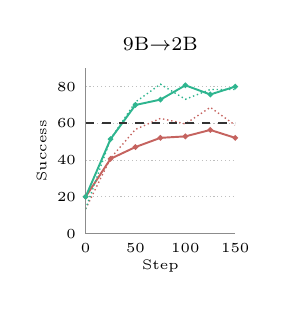
\begin{tikzpicture}
\begin{axis}[
  width=1.9cm, height=2.1cm, scale only axis,
  xmin=0, xmax=150, ymin=0, ymax=90, xtick={0,50,100,150}, ylabel={Success}, xlabel={Step},
  axis lines*=left, axis line style={black!45}, tick style={draw=none}, ytick pos=left,
  ymajorgrids, grid style={densely dotted, black!25}, every tick label/.append style={font=\tiny},
  ylabel style={font=\tiny, yshift=-3pt}, xlabel style={font=\tiny, yshift=4pt}, title style={font=\scriptsize, yshift=-3pt},
  title={9B$\to$2B},
]
\addplot[vanRed, line width=0.7pt, mark=*, mark size=0.6pt] coordinates {(0,20.0) (25,40.7) (50,47.1) (75,52.1) (100,52.9) (125,56.4) (150,52.1)};
\addplot[vanRed, densely dotted, line width=0.5pt] coordinates {(0,13.4) (25,41.0) (50,56.7) (75,62.7) (100,59.7) (125,68.7) (150,59.0)};
\addplot[r2sGreen, line width=0.7pt, mark=*, mark size=0.6pt] coordinates {(0,20.0) (25,51.4) (50,70.0) (75,72.9) (100,80.7) (125,75.7) (150,80.0)};
\addplot[r2sGreen, densely dotted, line width=0.5pt] coordinates {(0,13.4) (25,51.5) (50,71.6) (75,81.3) (100,73.1) (125,78.4) (150,78.4)};
\draw[dashed, black!80, line width=0.6pt] (rel axis cs:0,0.6693) -- (rel axis cs:1,0.6693);
\end{axis}
\end{tikzpicture}
\hfill
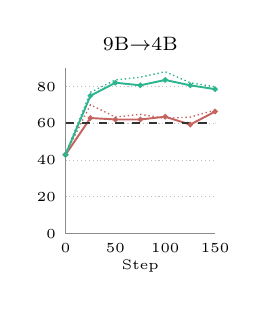
\begin{tikzpicture}
\begin{axis}[
  width=1.9cm, height=2.1cm, scale only axis,
  xmin=0, xmax=150, ymin=0, ymax=90, xtick={0,50,100,150},  xlabel={Step},
  axis lines*=left, axis line style={black!45}, tick style={draw=none}, ytick pos=left,
  ymajorgrids, grid style={densely dotted, black!25}, every tick label/.append style={font=\tiny},
  ylabel style={font=\tiny, yshift=-3pt}, xlabel style={font=\tiny, yshift=4pt}, title style={font=\scriptsize, yshift=-3pt},
  title={9B$\to$4B},
]
\addplot[vanRed, line width=0.7pt, mark=*, mark size=0.6pt] coordinates {(0,42.9) (25,62.9) (50,62.1) (75,62.1) (100,63.6) (125,59.3) (150,66.4)};
\addplot[vanRed, densely dotted, line width=0.5pt] coordinates {(0,43.3) (25,70.1) (50,63.4) (75,64.9) (100,62.7) (125,63.4) (150,67.2)};
\addplot[r2sGreen, line width=0.7pt, mark=*, mark size=0.6pt] coordinates {(0,42.9) (25,75.0) (50,82.1) (75,80.7) (100,83.6) (125,80.7) (150,78.6)};
\addplot[r2sGreen, densely dotted, line width=0.5pt] coordinates {(0,43.3) (25,76.9) (50,83.6) (75,85.1) (100,88.1) (125,82.1) (150,79.9)};
\draw[dashed, black!80, line width=0.6pt] (rel axis cs:0,0.6693) -- (rel axis cs:1,0.6693);
\end{axis}
\end{tikzpicture}
\hfill
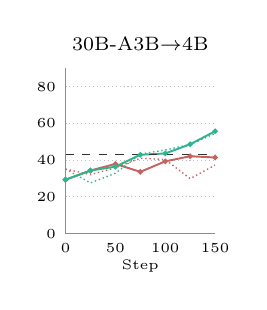
\begin{tikzpicture}
\begin{axis}[
  width=1.9cm, height=2.1cm, scale only axis,
  xmin=0, xmax=150, ymin=0, ymax=90, xtick={0,50,100,150},  xlabel={Step},
  axis lines*=left, axis line style={black!45}, tick style={draw=none}, ytick pos=left,
  ymajorgrids, grid style={densely dotted, black!25}, every tick label/.append style={font=\tiny},
  ylabel style={font=\tiny, yshift=-3pt}, xlabel style={font=\tiny, yshift=4pt}, title style={font=\scriptsize, yshift=-3pt},
  title={30B-A3B$\to$4B},
]
\addplot[vanRed, line width=0.7pt, mark=*, mark size=0.6pt] coordinates {(0,29.3) (25,34.3) (50,37.9) (75,33.6) (100,39.3) (125,42.1) (150,41.4)};
\addplot[vanRed, densely dotted, line width=0.5pt] coordinates {(0,35.1) (25,32.1) (50,35.8) (75,41.0) (100,40.3) (125,29.9) (150,37.3)};
\addplot[r2sGreen, line width=0.7pt, mark=*, mark size=0.6pt] coordinates {(0,29.3) (25,34.3) (50,36.4) (75,42.9) (100,43.6) (125,48.6) (150,55.7)};
\addplot[r2sGreen, densely dotted, line width=0.5pt] coordinates {(0,35.1) (25,27.6) (50,32.8) (75,43.3) (100,45.5) (125,48.5) (150,54.5)};
\draw[dashed, black!80, line width=0.6pt] (rel axis cs:0,0.4788) -- (rel axis cs:1,0.4788);
\end{axis}
\end{tikzpicture}
\hfill
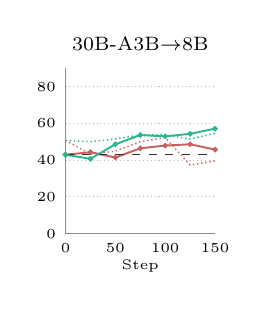
\begin{tikzpicture}
\begin{axis}[
  width=1.9cm, height=2.1cm, scale only axis,
  xmin=0, xmax=150, ymin=0, ymax=90, xtick={0,50,100,150},  xlabel={Step},
  axis lines*=left, axis line style={black!45}, tick style={draw=none}, ytick pos=left,
  ymajorgrids, grid style={densely dotted, black!25}, every tick label/.append style={font=\tiny},
  ylabel style={font=\tiny, yshift=-3pt}, xlabel style={font=\tiny, yshift=4pt}, title style={font=\scriptsize, yshift=-3pt},
  title={30B-A3B$\to$8B},
]
\addplot[vanRed, line width=0.7pt, mark=*, mark size=0.6pt] coordinates {(0,42.9) (25,44.3) (50,41.4) (75,46.4) (100,47.9) (125,48.6) (150,45.7)};
\addplot[vanRed, densely dotted, line width=0.5pt] coordinates {(0,50.7) (25,43.3) (50,44.8) (75,50.0) (100,52.2) (125,37.3) (150,39.6)};
\addplot[r2sGreen, line width=0.7pt, mark=*, mark size=0.6pt] coordinates {(0,42.9) (25,40.7) (50,48.6) (75,53.6) (100,52.9) (125,54.3) (150,57.1)};
\addplot[r2sGreen, densely dotted, line width=0.5pt] coordinates {(0,50.7) (25,50.0) (50,51.5) (75,53.7) (100,53.7) (125,51.5) (150,54.5)};
\draw[dashed, black!80, line width=0.6pt] (rel axis cs:0,0.4788) -- (rel axis cs:1,0.4788);
\end{axis}
\end{tikzpicture}
\hfill
\\[3pt]
\makebox[\linewidth][c]{\textbf{WebShop}}\\[1pt]
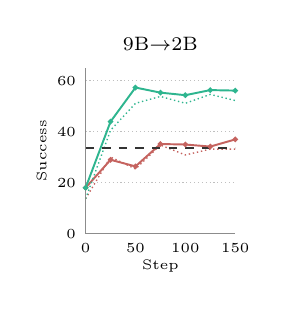
\begin{tikzpicture}
\begin{axis}[
  width=1.9cm, height=2.1cm, scale only axis,
  xmin=0, xmax=150, ymin=0, ymax=65, xtick={0,50,100,150}, ylabel={Success}, xlabel={Step},
  axis lines*=left, axis line style={black!45}, tick style={draw=none}, ytick pos=left,
  ymajorgrids, grid style={densely dotted, black!25}, every tick label/.append style={font=\tiny},
  ylabel style={font=\tiny, yshift=-3pt}, xlabel style={font=\tiny, yshift=4pt}, title style={font=\scriptsize, yshift=-3pt},
  title={9B$\to$2B},
]
\addplot[vanRed, line width=0.7pt, mark=*, mark size=0.6pt] coordinates {(0,18.0) (25,29.0) (50,26.4) (75,35.2) (100,35.0) (125,34.2) (150,37.0)};
\addplot[vanRed, densely dotted, line width=0.5pt] coordinates {(0,13.7) (25,30.1) (50,25.4) (75,34.8) (100,30.9) (125,33.2) (150,33.2)};
\addplot[r2sGreen, line width=0.7pt, mark=*, mark size=0.6pt] coordinates {(0,18.0) (25,44.0) (50,57.4) (75,55.4) (100,54.4) (125,56.4) (150,56.2)};
\addplot[r2sGreen, densely dotted, line width=0.5pt] coordinates {(0,13.7) (25,40.6) (50,51.2) (75,53.9) (100,51.2) (125,54.7) (150,52.3)};
\draw[dashed, black!80, line width=0.6pt] (rel axis cs:0,0.5159) -- (rel axis cs:1,0.5159);
\end{axis}
\end{tikzpicture}
\hfill
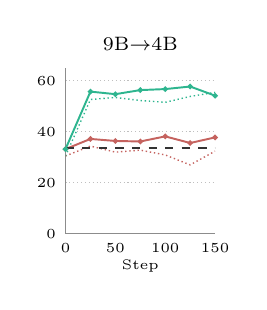
\begin{tikzpicture}
\begin{axis}[
  width=1.9cm, height=2.1cm, scale only axis,
  xmin=0, xmax=150, ymin=0, ymax=65, xtick={0,50,100,150},  xlabel={Step},
  axis lines*=left, axis line style={black!45}, tick style={draw=none}, ytick pos=left,
  ymajorgrids, grid style={densely dotted, black!25}, every tick label/.append style={font=\tiny},
  ylabel style={font=\tiny, yshift=-3pt}, xlabel style={font=\tiny, yshift=4pt}, title style={font=\scriptsize, yshift=-3pt},
  title={9B$\to$4B},
]
\addplot[vanRed, line width=0.7pt, mark=*, mark size=0.6pt] coordinates {(0,33.2) (25,37.2) (50,36.4) (75,36.2) (100,38.2) (125,35.6) (150,37.8)};
\addplot[vanRed, densely dotted, line width=0.5pt] coordinates {(0,30.5) (25,34.4) (50,32.0) (75,32.8) (100,30.9) (125,27.0) (150,32.4)};
\addplot[r2sGreen, line width=0.7pt, mark=*, mark size=0.6pt] coordinates {(0,33.2) (25,55.8) (50,54.8) (75,56.4) (100,56.8) (125,57.8) (150,54.2)};
\addplot[r2sGreen, densely dotted, line width=0.5pt] coordinates {(0,30.5) (25,52.7) (50,53.5) (75,52.3) (100,51.6) (125,53.9) (150,55.5)};
\draw[dashed, black!80, line width=0.6pt] (rel axis cs:0,0.5159) -- (rel axis cs:1,0.5159);
\end{axis}
\end{tikzpicture}
\hfill
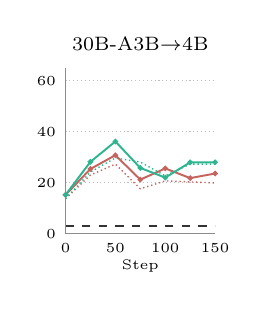
\begin{tikzpicture}
\begin{axis}[
  width=1.9cm, height=2.1cm, scale only axis,
  xmin=0, xmax=150, ymin=0, ymax=65, xtick={0,50,100,150},  xlabel={Step},
  axis lines*=left, axis line style={black!45}, tick style={draw=none}, ytick pos=left,
  ymajorgrids, grid style={densely dotted, black!25}, every tick label/.append style={font=\tiny},
  ylabel style={font=\tiny, yshift=-3pt}, xlabel style={font=\tiny, yshift=4pt}, title style={font=\scriptsize, yshift=-3pt},
  title={30B-A3B$\to$4B},
]
\addplot[vanRed, line width=0.7pt, mark=*, mark size=0.6pt] coordinates {(0,15.2) (25,25.4) (50,30.8) (75,21.2) (100,25.6) (125,21.8) (150,23.6)};
\addplot[vanRed, densely dotted, line width=0.5pt] coordinates {(0,13.7) (25,23.0) (50,27.3) (75,17.6) (100,20.7) (125,20.3) (150,19.9)};
\addplot[r2sGreen, line width=0.7pt, mark=*, mark size=0.6pt] coordinates {(0,15.2) (25,28.2) (50,36.2) (75,25.8) (100,22.0) (125,28.0) (150,28.0)};
\addplot[r2sGreen, densely dotted, line width=0.5pt] coordinates {(0,13.7) (25,24.2) (50,29.7) (75,28.1) (100,22.7) (125,27.3) (150,27.3)};
\draw[dashed, black!80, line width=0.6pt] (rel axis cs:0,0.0441) -- (rel axis cs:1,0.0441);
\end{axis}
\end{tikzpicture}
\hfill
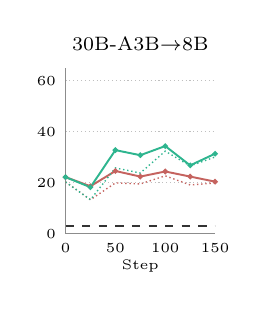
\begin{tikzpicture}
\begin{axis}[
  width=1.9cm, height=2.1cm, scale only axis,
  xmin=0, xmax=150, ymin=0, ymax=65, xtick={0,50,100,150},  xlabel={Step},
  axis lines*=left, axis line style={black!45}, tick style={draw=none}, ytick pos=left,
  ymajorgrids, grid style={densely dotted, black!25}, every tick label/.append style={font=\tiny},
  ylabel style={font=\tiny, yshift=-3pt}, xlabel style={font=\tiny, yshift=4pt}, title style={font=\scriptsize, yshift=-3pt},
  title={30B-A3B$\to$8B},
]
\addplot[vanRed, line width=0.7pt, mark=*, mark size=0.6pt] coordinates {(0,22.2) (25,18.6) (50,24.6) (75,22.4) (100,24.4) (125,22.4) (150,20.4)};
\addplot[vanRed, densely dotted, line width=0.5pt] coordinates {(0,20.3) (25,13.3) (50,19.9) (75,19.5) (100,22.7) (125,19.1) (150,19.9)};
\addplot[r2sGreen, line width=0.7pt, mark=*, mark size=0.6pt] coordinates {(0,22.2) (25,18.2) (50,32.8) (75,30.8) (100,34.4) (125,26.8) (150,31.4)};
\addplot[r2sGreen, densely dotted, line width=0.5pt] coordinates {(0,20.3) (25,13.3) (50,25.8) (75,23.8) (100,32.4) (125,26.6) (150,30.1)};
\draw[dashed, black!80, line width=0.6pt] (rel axis cs:0,0.0441) -- (rel axis cs:1,0.0441);
\end{axis}
\end{tikzpicture}
\hfill
\\[3pt]
\makebox[\linewidth][c]{\textbf{ScienceWorld}}\\[1pt]
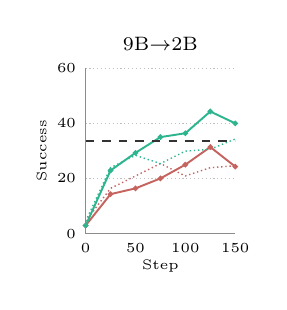
\begin{tikzpicture}
\begin{axis}[
  width=1.9cm, height=2.1cm, scale only axis,
  xmin=0, xmax=150, ymin=0, ymax=60, xtick={0,50,100,150}, ylabel={Success}, xlabel={Step},
  axis lines*=left, axis line style={black!45}, tick style={draw=none}, ytick pos=left,
  ymajorgrids, grid style={densely dotted, black!25}, every tick label/.append style={font=\tiny},
  ylabel style={font=\tiny, yshift=-3pt}, xlabel style={font=\tiny, yshift=4pt}, title style={font=\scriptsize, yshift=-3pt},
  title={9B$\to$2B},
]
\addplot[vanRed, line width=0.7pt, mark=*, mark size=0.6pt] coordinates {(0,2.9) (25,14.3) (50,16.4) (75,20.0) (100,25.0) (125,31.4) (150,24.3)};
\addplot[vanRed, densely dotted, line width=0.5pt] coordinates {(0,4.5) (25,16.4) (50,20.9) (75,25.4) (100,20.9) (125,23.9) (150,24.6)};
\addplot[r2sGreen, line width=0.7pt, mark=*, mark size=0.6pt] coordinates {(0,2.9) (25,22.9) (50,29.3) (75,35.0) (100,36.4) (125,44.3) (150,40.0)};
\addplot[r2sGreen, densely dotted, line width=0.5pt] coordinates {(0,4.5) (25,23.9) (50,28.4) (75,25.4) (100,29.9) (125,30.6) (150,34.3)};
\draw[dashed, black!80, line width=0.6pt] (rel axis cs:0,0.5595) -- (rel axis cs:1,0.5595);
\end{axis}
\end{tikzpicture}
\hfill
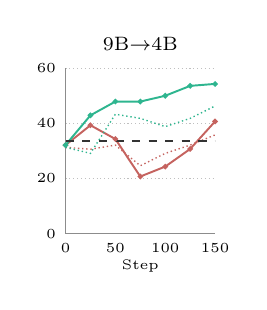
\begin{tikzpicture}
\begin{axis}[
  width=1.9cm, height=2.1cm, scale only axis,
  xmin=0, xmax=150, ymin=0, ymax=60, xtick={0,50,100,150},  xlabel={Step},
  axis lines*=left, axis line style={black!45}, tick style={draw=none}, ytick pos=left,
  ymajorgrids, grid style={densely dotted, black!25}, every tick label/.append style={font=\tiny},
  ylabel style={font=\tiny, yshift=-3pt}, xlabel style={font=\tiny, yshift=4pt}, title style={font=\scriptsize, yshift=-3pt},
  title={9B$\to$4B},
]
\addplot[vanRed, line width=0.7pt, mark=*, mark size=0.6pt] coordinates {(0,32.1) (25,39.3) (50,34.3) (75,20.7) (100,24.3) (125,30.7) (150,40.7)};
\addplot[vanRed, densely dotted, line width=0.5pt] coordinates {(0,31.3) (25,30.6) (50,32.1) (75,24.6) (100,29.1) (125,32.1) (150,35.8)};
\addplot[r2sGreen, line width=0.7pt, mark=*, mark size=0.6pt] coordinates {(0,32.1) (25,42.9) (50,47.9) (75,47.9) (100,50.0) (125,53.6) (150,54.3)};
\addplot[r2sGreen, densely dotted, line width=0.5pt] coordinates {(0,31.3) (25,29.1) (50,43.3) (75,41.8) (100,38.8) (125,41.8) (150,46.3)};
\draw[dashed, black!80, line width=0.6pt] (rel axis cs:0,0.5595) -- (rel axis cs:1,0.5595);
\end{axis}
\end{tikzpicture}
\hfill
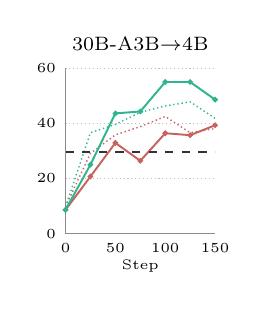
\begin{tikzpicture}
\begin{axis}[
  width=1.9cm, height=2.1cm, scale only axis,
  xmin=0, xmax=150, ymin=0, ymax=60, xtick={0,50,100,150},  xlabel={Step},
  axis lines*=left, axis line style={black!45}, tick style={draw=none}, ytick pos=left,
  ymajorgrids, grid style={densely dotted, black!25}, every tick label/.append style={font=\tiny},
  ylabel style={font=\tiny, yshift=-3pt}, xlabel style={font=\tiny, yshift=4pt}, title style={font=\scriptsize, yshift=-3pt},
  title={30B-A3B$\to$4B},
]
\addplot[vanRed, line width=0.7pt, mark=*, mark size=0.6pt] coordinates {(0,8.6) (25,20.7) (50,32.9) (75,26.4) (100,36.4) (125,35.7) (150,39.3)};
\addplot[vanRed, densely dotted, line width=0.5pt] coordinates {(0,9.7) (25,29.1) (50,35.8) (75,38.8) (100,42.5) (125,36.6) (150,38.1)};
\addplot[r2sGreen, line width=0.7pt, mark=*, mark size=0.6pt] coordinates {(0,8.6) (25,25.0) (50,43.6) (75,44.3) (100,55.0) (125,55.0) (150,48.6)};
\addplot[r2sGreen, densely dotted, line width=0.5pt] coordinates {(0,9.7) (25,36.6) (50,39.6) (75,44.0) (100,46.3) (125,47.8) (150,41.8)};
\draw[dashed, black!80, line width=0.6pt] (rel axis cs:0,0.4921) -- (rel axis cs:1,0.4921);
\end{axis}
\end{tikzpicture}
\hfill
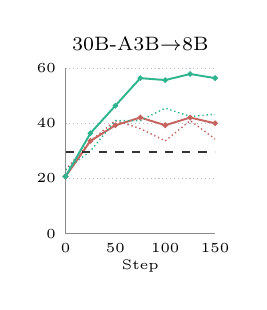
\begin{tikzpicture}
\begin{axis}[
  width=1.9cm, height=2.1cm, scale only axis,
  xmin=0, xmax=150, ymin=0, ymax=60, xtick={0,50,100,150},  xlabel={Step},
  axis lines*=left, axis line style={black!45}, tick style={draw=none}, ytick pos=left,
  ymajorgrids, grid style={densely dotted, black!25}, every tick label/.append style={font=\tiny},
  ylabel style={font=\tiny, yshift=-3pt}, xlabel style={font=\tiny, yshift=4pt}, title style={font=\scriptsize, yshift=-3pt},
  title={30B-A3B$\to$8B},
]
\addplot[vanRed, line width=0.7pt, mark=*, mark size=0.6pt] coordinates {(0,20.7) (25,33.6) (50,39.3) (75,42.1) (100,39.3) (125,42.1) (150,40.0)};
\addplot[vanRed, densely dotted, line width=0.5pt] coordinates {(0,23.1) (25,33.6) (50,41.0) (75,38.1) (100,33.6) (125,41.0) (150,34.3)};
\addplot[r2sGreen, line width=0.7pt, mark=*, mark size=0.6pt] coordinates {(0,20.7) (25,36.4) (50,46.4) (75,56.4) (100,55.7) (125,57.9) (150,56.4)};
\addplot[r2sGreen, densely dotted, line width=0.5pt] coordinates {(0,23.1) (25,29.9) (50,41.0) (75,41.0) (100,45.5) (125,42.5) (150,43.3)};
\draw[dashed, black!80, line width=0.6pt] (rel axis cs:0,0.4921) -- (rel axis cs:1,0.4921);
\end{axis}
\end{tikzpicture}
\hfill
\\[3pt]
{\tiny \tikz[baseline=-0.4ex]{\draw[vanRed, line width=0.7pt] (0,0.065) -- (0.4,0.065);}\,Vanilla OPD\quad \tikz[baseline=-0.4ex]{\draw[r2sGreen, line width=0.7pt] (0,0.065) -- (0.4,0.065);}\,\method{}\quad Solid: seen / canonical\quad Dotted: unseen / pool\quad \tikz[baseline=-0.4ex]{\draw[dashed, black!80, line width=0.6pt] (0,0.065) -- (0.4,0.065);}\,Teacher Alone}
\caption{\textbf{Success over training in every cell of \Cref{tab:main}.} Vanilla and \method{} students, one decode every 25 updates (update 0: untrained). Solid: seen split or WebShop's canonical goals; dotted: unseen split or its 256-goal pool; dashed: the teacher acting alone on the seen split.}
\label{fig:curves-all}
\end{figure}


\textbf{Training curves complement the final-checkpoint comparison.} \Cref{fig:curves-all} plots the in-training evaluation of the vanilla and \method{} students of every cell of \Cref{tab:main}: one decode every 25 updates under the training seed, so the final point of each curve is the first of the three decodes behind the table. The \method{} student ends above vanilla OPD in all twelve cells, on both splits, and above the teacher acting alone on the seen split in all twelve, with no checkpoint selection.

\textbf{Three training runs per method.} \Cref{fig:teacher-bars} follows vanilla OPD, TCOD-F2B, Guided-OPD, FutureBridge and \method{} from the Qwen3.5-9B teacher to the Qwen3.5-4B student under the protocol of \Cref{app:protocol}. Each method has three training runs per environment, started from the same untrained student and differing only in the training seed; the three \method{} runs share the one repaired teacher of \Cref{tab:main}, so its band reflects student training alone. Each run is evaluated every 25 updates under its own seed, update 0 being the untrained student common to all five curves. Lines are means over the three runs and bands one sample standard deviation, without interpolation or checkpoint selection; the dashed line is the teacher acting alone.
